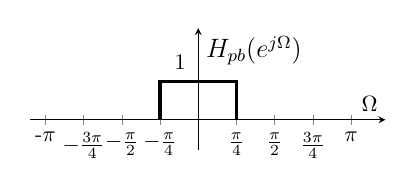
\begin{tikzpicture}[scale=0.8,transform shape]
    \begin{axis}[
        x=0.05\textwidth,y=0.05\textwidth,
        axis y line=center,
        axis x line=middle,
        xlabel=$\Omega$,ylabel={\large $H_{pb}(e^{j\Omega})$},
        xmin=-4.4,xmax=4.9,
        ymin=-0.8,ymax=2.4,
        xtick = {-4, -3, -2, -1, 0, 1, 2, 3, 4},
        xticklabels = {-$\pi$, $-\frac{3\pi}{4}$, $-\frac{\pi}{2}$, $-\frac{\pi}{4}$, $0$, $\frac{\pi}{4}$, $\frac{\pi}{2}$, $\frac{3\pi}{4}$, $\pi$},
        ytick = {0, 1},
        yticklabels = {$0$,$1$},
        yticklabel style={yshift=0.3cm},
        ]

        \addplot[
        black,
        ultra thick
        ] coordinates {
            (-1,0) (-1,1) (1,1) (1,0)
        } ;
    \end{axis}
\end{tikzpicture}